\chapter{Results} 
  The main results of this thesis are give here:
    the cross section for coherent \JPsi~production, the incoherent \JPsi~cross
    section, the cross section for muon pairs from photon-photon interactions,
    the ratio between break up mode yields, and the rapidity correlations 
    between dimuon candidates and neutrons in the ZDC.

  \section{Coherent cross section}
  The coherent cross section in calculated from the following equation:
  \begin{equation}
    \frac{d\sigma^{J/\psi}_{co}}{dy}  = \frac{N_{cor} f_{co}  }
    { \Delta y\mathcal{L}_{int} \varepsilon_{ZDC} \varepsilon_{p_{T}} 
      BR_{\mu^{+}\mu^{-}}}
    \label{eq:expXSecCo}
   \end{equation}
   where $N_{cor}$ is corrected dimuon yield, $f_{co}$ is the 
     fraction of events that come from the coherent process, 
     $BR_{\mu^{+}\mu^{-}}$ is the branching ratio for \JPsi~to $\mu^{+}\mu^{-}$, 
     $\varepsilon_{ZDC}$ is the efficiency for triggering the ZDC, 
     $\varepsilon_{p_{T}}$ is the efficiency for the 0.15 GeV cut in $p_{T}$, 
     $\mathcal{L}_{int}$ is the integrated luminosity, and $\Delta y$ is the 
     width the rapidity interval.

  The raw yield of dimuon candidates was measured after applying the cuts 
    described in Section~\ref{sec:DataSetEvSel}.
  \begin{figure}[!Hhtb]
    \centering
    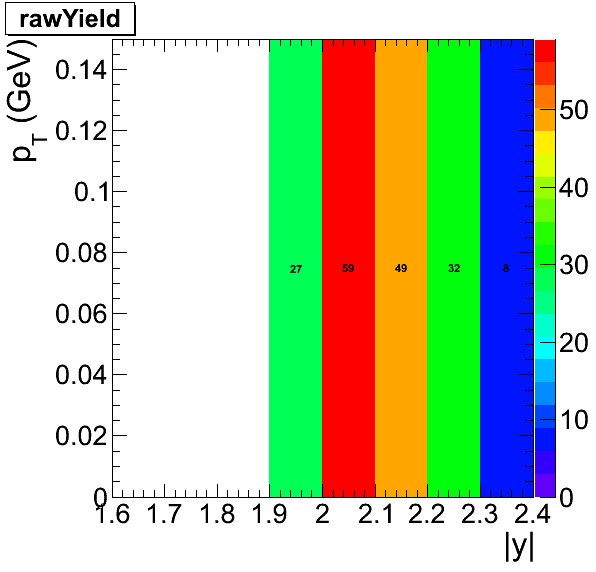
\includegraphics[width=0.6\textwidth]{rawYield}
    \caption{Raw yield for the Coherent cross section measurement.}
    \label{fig:rawYieldCo}
  \end{figure}
  $N_{cor}$ was calculated by dividing the raw yields from 
    Fig.~\ref{fig:rawYieldCo} by the acceptance and efficiency factor from 
    Fig.~\ref{fig:avAccEff}, which combines $A$ and 
    $\varepsilon^{dimuon}_{trigger}$ as described in Section.~\ref{sec:effDet}.
  The corrected yields, $N_{cor}$, are shown in Fig.~\ref{fig:corYieldCo}.
  \begin{figure}[!Hhtb]
    \centering
    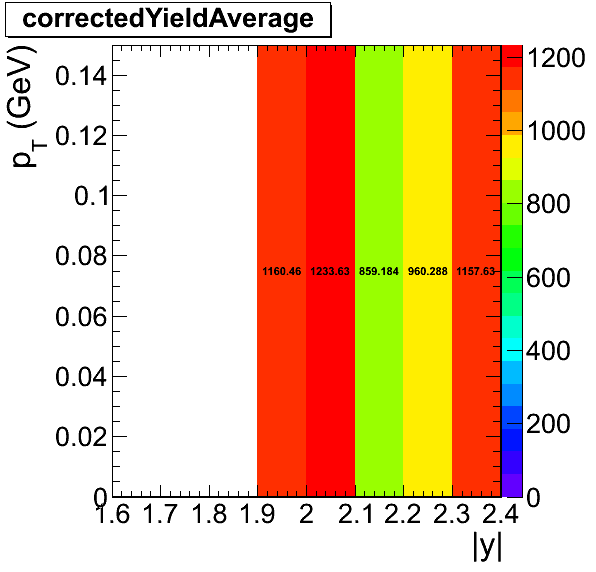
\includegraphics[width=0.6\textwidth]{correctedYieldAverage}
    \caption{Corrected yields for the coherent p$_{T}$ region.}
    \label{fig:corYieldCo}
  \end{figure}
  For the coherent cross section measurement, $N_{cor}$ is taken from the 
    region 2.0 < $|y|$ < 2.2 and $p_{T}$ < 0.15 GeV to avoid the edges of the
    detectors acceptance, bin migration in the calculation of $A$, and overlap
    between the coherent and incoherent process.
  From this procedure, the $N_{cor}$ was measured to be 1903.
  
  To measure $f_{co}$, the simultaneous fit shown in 
    Fig.~\ref{fig:simFitMassPtGauss} was used.
  The normalizations for each of the three components to the signal are fixed 
  by the fit as described in Section~\ref{sec:sigEx}.
  The normalized coherent template is integrated up to 0.15 GeV in $p_{T}$ and
    divided by the integral of the data $p_{T}$ spectrum up to 0.15 GeV.
  The statistical error taken from the fit, $f_{co}$ = 0.60 $\pm$ 0.11.

  The two efficiency terms, $\varepsilon_{ZDC}$ and $\varepsilon_{p_{T}}$, were
    measured from data and MC respectively.
  As described in Section~\ref{sec:breakUpDet}, $\varepsilon_{ZDC}$ was 
    measured in the from the ZDC triggered data set by dividing the number of 
    events both fire the ZDC trigger and pass the one neutron threshold.
  $\varepsilon_{ZDC}$ was measured to be 0.96 with a negligible statistical 
    error.
  The efficiency of the 0.15 GeV $p_{T}$ cut was estimated from MC by dividing 
    the number of events that are lost by applying the $p_{T}$ cut after all
    other cuts are applied. 
  From this method $\varepsilon_{p_{T}}$ = 0.95.
  
  The remaining two terms, $\mathcal{L}_{int}$ and $BR_{\mu^{+}\mu^{-}}$, 
    depend on Ref.~\cite{cmsLumi} and Ref.~\cite{pdg}.
  Ref.~\cite{cmsLumi} describes the method of using activity in HF to measure 
    the luminosity. 
  From this method, $\mathcal{L}_{int}$ was measured to be 143.3$\mu b^{-1}\pm$7.2.
  $BR_{\mu^{+}\mu^{-}}$ from Ref.~\cite{pdg} is 0.0593 $\pm$ 0.0006.
  From Equation~\ref{eq:expXSecCo}, $\frac{d\sigma^{J/\psi}_{co}}{dy}$ = 368 $mb$.

  \section{Incoherent cross section}
  The same basic procedure for measuring the coherent cross section was used to 
    calculate the incoherent cross section.  
  \section{Break up ratios}
    In Table~\ref{tab:r2} the ratio between raw yields for different break up 
      modes are shown.
    \begin{figure}[!Hhtb]
      \centering
      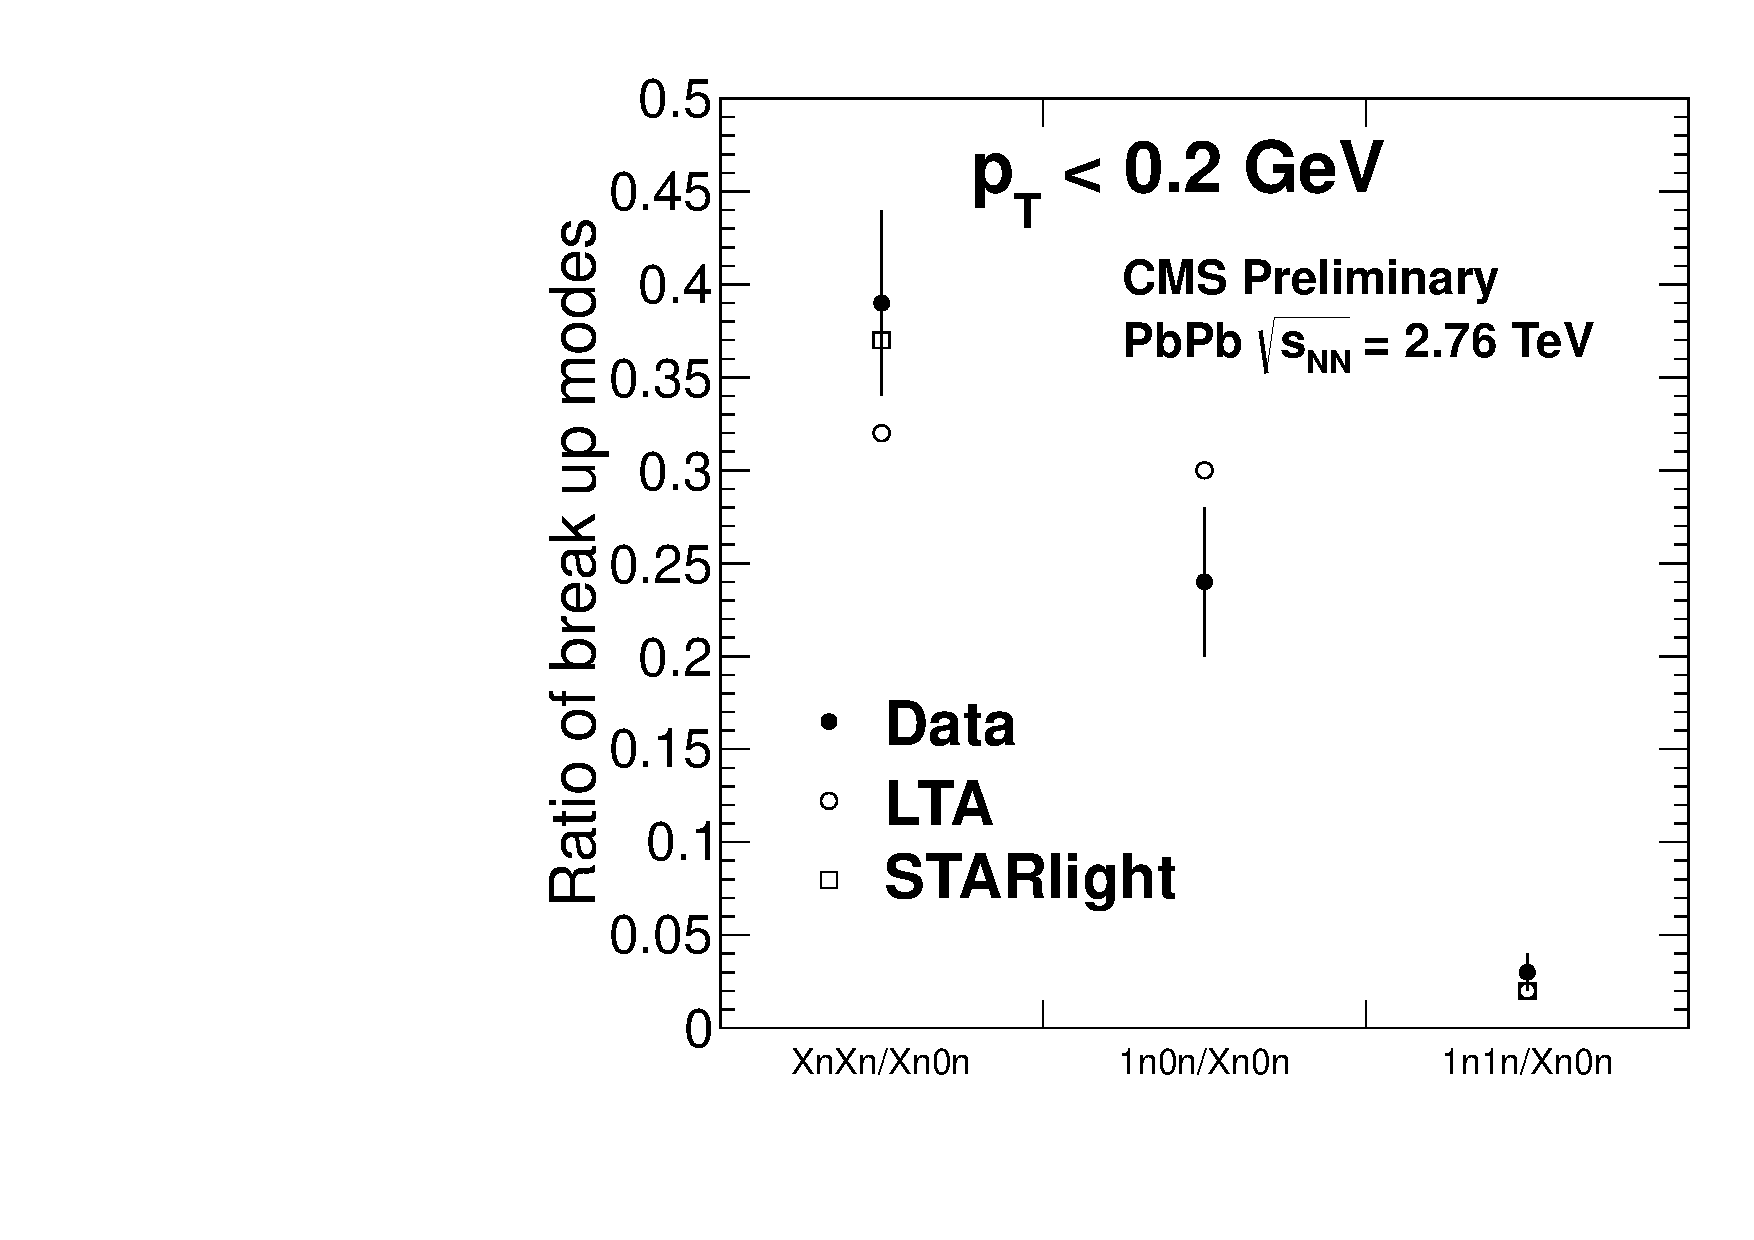
\includegraphics[width=.6\textwidth]{coherentBreakup}
      \caption{Ratio between J/$\psi$ yeilds XnXn and 1n0n break-up modes 
        compared the Xn0n break-up mode for J/$\psi$ with $p_{T}$ below 150 
        MeV.}
      \label{fig:coherentBreakUp}
    \end{figure}
   
    Fig.~\ref{fig:coherentBreakUp} and Fig.~\ref{fig:incoherentBreakUp} compare
      the raw break up ratios two STARlight and LTA predictions. 
    \begin{figure}[!Hhtb]
      \centering
      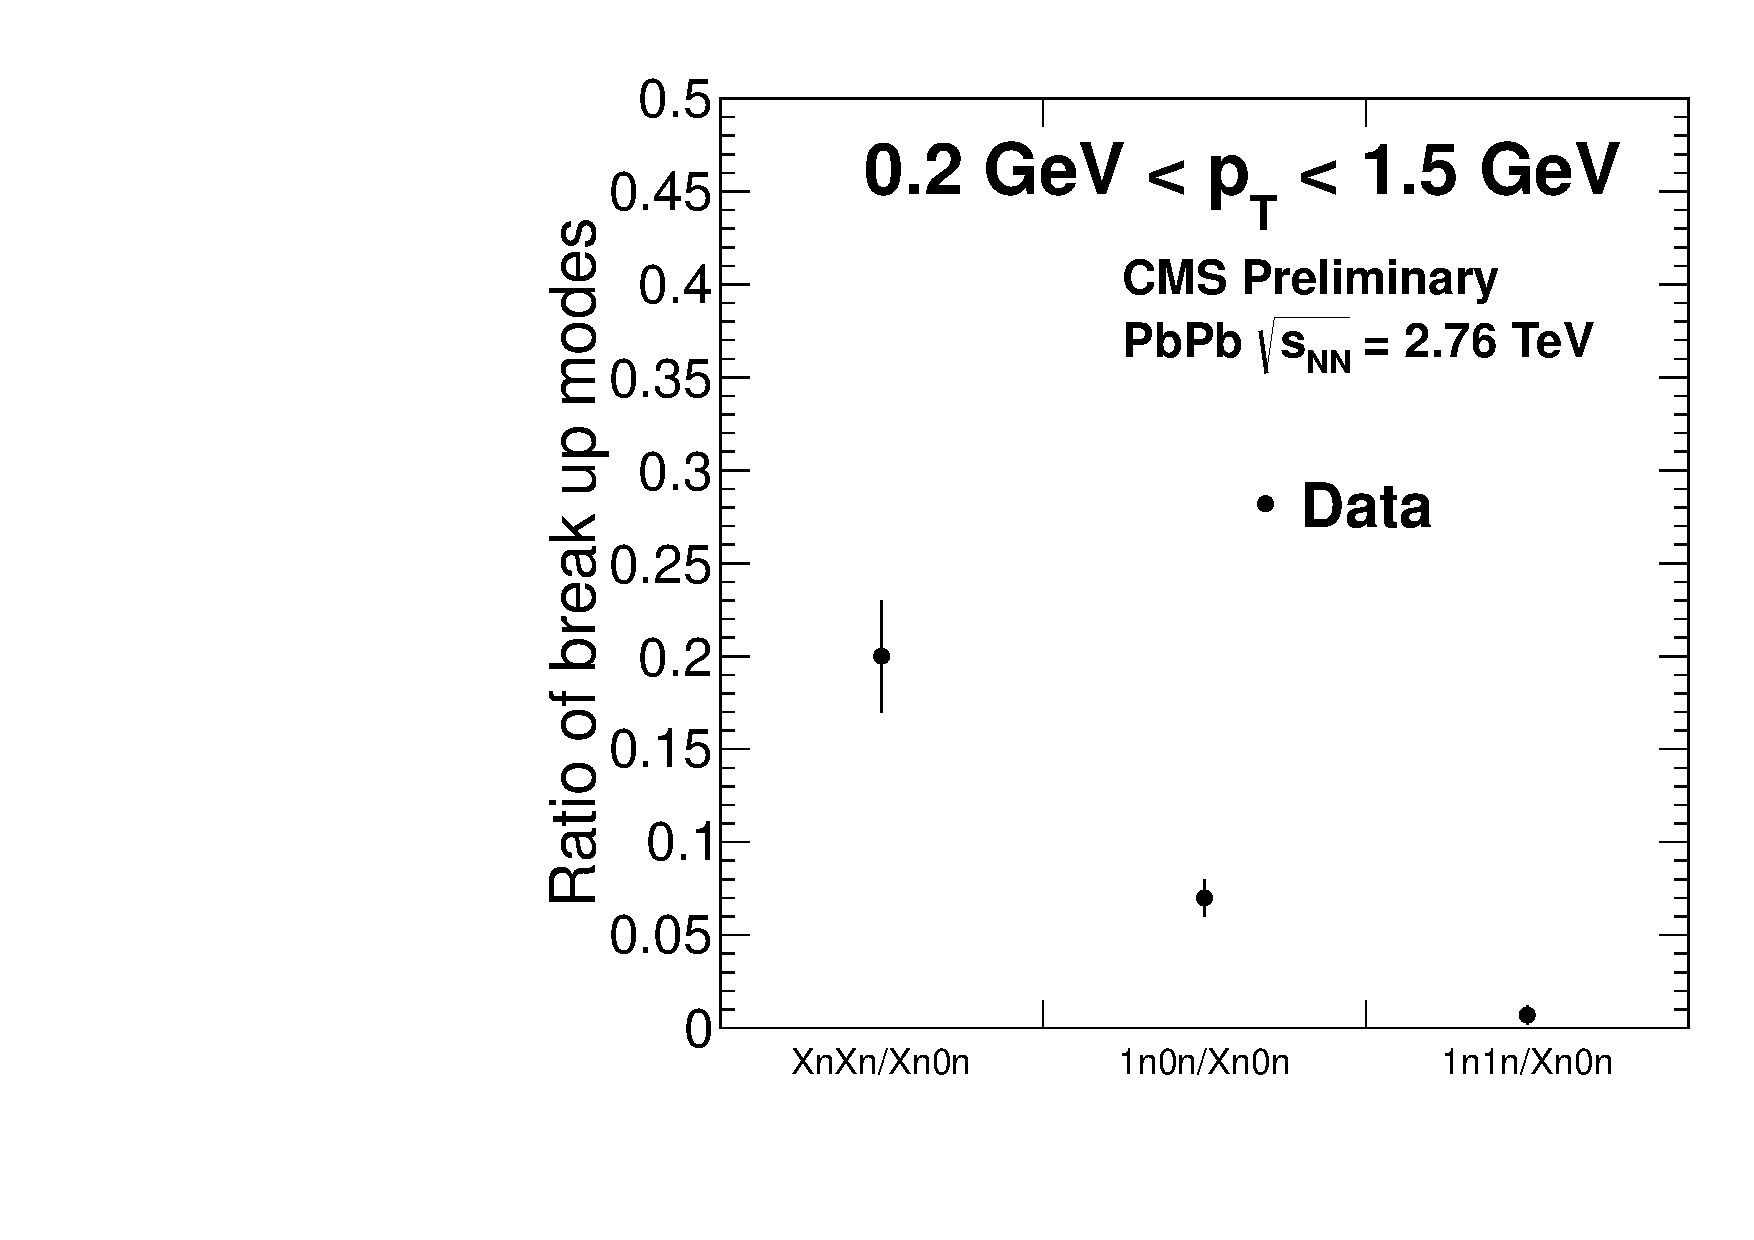
\includegraphics[width=.6\textwidth]{incoherentBreakup}
      \caption{Ratio between J/$\psi$ yeilds XnXn and 1n0n break-up modes 
        compared the Xn0n break-up mode for J/$\psi$ with 0.2 $< p_{T} <$ 
        1.5 GeV.}
      \label{fig:incoherentBreakUp}
    \end{figure}

    The number of the coherent and incoherent J/$\psi$ for each break-up mode are
      given in the Tab.~\ref{tab:r1}. 
    The ratios between the modes X$_{n}$X$_{n}$, 1$_{n}$0$_{n}$, 1$_{n}$1$_{n}$ and
      the mode  X$_{n}$0$_{n}$ are given in the table Tab.~\ref{tab:r2}. 
    Some of the  ratios can be obtained from  {\sc starlight} and from the Zhalov 
      and thus are given in Tab.~\ref{tab:r3}.
    \begin{table}[h]
      \begin{center}
      \begin{tabular}{|c|c|c|c|c|c|}
        \hline
         &  X$_{n}$0$_{n}$& X$_{n}$X$_{n}$ & 1$_{n}$0$_{n}$ & 1$_{n}$1$_{n}$  \\ \hline
        coherent J/$\psi$ &  242$\pm$16&94$\pm$10&58$\pm$8&8$\pm$3\\ \hline
        incoherent J/$\psi$ & 291$\pm$17&57$\pm$8&19$\pm$4&2$\pm$1\\ \hline
      \end{tabular}
      \caption{\label{tab:r1} Number of coherent J/$\psi$ integrated over $p_{T}$ and $y$ 
        with statistical uncertainty.}
      \end{center}
    \end{table}
    
    \begin{table}[h]
      \begin{center}
        \begin{tabular}{|c|c|c|c|c|}
          \hline
          & X$_{n}$X$_{n}$/X$_{n}$0$_{n}$ & 1$_{n}$0$_{n}$/X$_{n}$0$_{n}$ & 1$_{n}$1$_{n}$/X$_{n}$0$_{n}$  \\ \hline
          coherent J/$\psi$ &  0.39$\pm$0.05&0.24$\pm$0.04&0.03$\pm$0.01\\ \hline
          incoherent J/$\psi$ &  0.20$\pm$0.03&0.07$\pm$0.02&0.007$\pm$0.005 \\ \hline
        \end{tabular}
      \caption{\label{tab:r2} Number of coherent J/$\psi$ integrated over $p_{T}$ and $y$ 
        with statistical uncertainty.}
      \end{center}
    \end{table}

    In Table~\ref{tab:r3} the ratio between break up modes are shown for 
      different theories and processes.
    \begin{table}[h]
      \begin{center}
        \begin{tabular}{|c|c|c|c|c|}
          \hline
          & X$_{n}$X$_{n}$/X$_{n}$0$_{n}$ & 1$_{n}$0$_{n}$/X$_{n}$0$_{n}$ & 1$_{n}$1$_{n}$/X$_{n}$0$_{n}$  \\ \hline
          STARlight coherent &  0.37&-&0.02\\ \hline
          Zhalov coherent& 0.32&0.30&0.02\\ \hline
          STARlight incoherent &  0.37&-&0.007$\pm$0.02 \\ \hline
        \end{tabular}
        \caption{\label{tab:r3} Number of  J/$\psi$ integrated over $p_{T}$ and $y$ with 
          statistical uncertainty.}
      \end{center}
    \end{table}

  \section{diMuon-neutron correlations}
    In this section the correlation between the rapidity of the $\mu^{+}\mu^{-}$ 
      and of the neutron is studied. The following samples are studied: 
    \begin{itemize}
      \item $\gamma + A$ collisions in which two cases are considered
      \begin{itemize}
        \item elastic coherent interaction: here photon interacts with entier
          nucleus coherently and produce \JPsi. 
          Another photon is needed to cause the breakup and neutron emission. 
          Those two photons are uncorrelated and thus we don't expect to 
            observe the correlation between the rapidity of the neutron and the
            rapidity of the \JPsi.
          In the data sample this corresponds to the low-\pt \JPsi 
            (\pt$<$0.15~GeV). 
        \item inelastic incoherent interaction: here a single high \pt photoni
          interacting with nucleus produce the \JPsi and neutron. 
          The correlation between the rapidity of the neutron and the rapidity
            of the \JPsi is expected.
          In the data sample this corresponds to the high-\pt \JPsi 
            (0.15$<$\pt$<$1.05). 
      \end{itemize}
      \item $\gamma \gamma$ collisions: two photons collide and produce the 
        $\mu^{+}\mu^{-}$  and the third photon is needed to excite one of
          the nucleons and produce neutron. 
        Thus we don't expect to see the correlation between the rapidity of the
          neutron and the rapidity of the $\mu^{+}\mu^{-}$. 
        In the data sample this corresponds to the $\mu^{+}\mu^{-}$ with the
          invariant mass between 4 and 8~GeV. 
    \end{itemize}

    In order to study the correlation in rapidity between the neutron and
      dimuon direction we below four quantities and give they values in 
      Table~\ref{tab:corrneutronjpsi}.  
    \begin{itemize}
      \item $y^{-}_{\mu\mu} \wedge y_{n}^{-}$: number of $\mu^{+}\mu^{-}$ having
         $y<0$ and the neutron in ZDC$^{-}$ ($y<0$)
      \item $y^{-}_{\mu\mu} \wedge y_{n}^{+}$: number of $\mu^{+}\mu^{-}$ having
         $y<0$ and the neutron in ZDC$^{+}$ ($y>0$)
      \item $y^{+}_{\mu\mu} \wedge y_{n}^{+}$: number of $\mu^{+}\mu^{-}$ having
         $y>0$ and the neutron in ZDC$^{+}$ ($y>0$)
      \item $y^{+}_{\mu\mu} \wedge y_{n}^{-}$: number of $\mu^{+}\mu^{-}$ having
         $y>0$ and the neutron in ZDC$^{-}$ ($y<0$)
    \end{itemize}

    The ratio $R_{opp/same}$ is defined as: 
    \begin{equation}
      R_{opp/same} = \frac{y^{-}_{\mu\mu} \wedge y_{n}^{+} + y^{+}_{\mu\mu} 
        \wedge y_{n}^{-}}{y^{-}_{\mu\mu} \wedge y_{n}^{-} + y^{+}_{\mu\mu} 
        \wedge y_{n}^{+}}
    \end{equation}
    
    Ratios studied in this section are only sensitive to the difference between
      the ZDC$^{-}$ and ZDC$^{-}$.
    It is seen that the efficiency of both ZDCs in not exactly the same i.e.
      the efficiencies of ZDC$^{-}$ and ZDC$^{+}$ are respectively 
      $\varepsilon_{ZDC^{-}}$=0.98 and  $\varepsilon_{ZDC^{+}}$=0.94 and this 
      is taken in the account in the estimations. 
    The $R_{opp/same}$ radio corrected by the ZDCs efficiencies is also 
      included in Table~\ref{tab:corrneutronjpsi} and called 
      $R_{opp/same}^{\varepsilon_{ZDC}}$. 
    It is seen that the difference between corrected and uncorrected results is
      very small. 
    Other uncertainties cancel. 
    In this case cuts related to the acceptance and efficiencies corrections 
      are not necessary and thus they are released.
    
    Figure~\ref{fig:PtcorrandRation} gives \pt distributions of the \JPsi 
      when \JPsi and neutron have the opposite rapidity direction or when they 
      have the same rapidity direction for low-\pt and high-\pt \JPsi. 
    Also the Fig~\ref{fig:PtcorrandRation} gives the $R_{opp/same}$ for low-\pt
      and high-\pt \JPsi. 
    In is send from this plot that in the case of the low-\pt \JPsi this 
      $R_{opp/same}$ ratio is close to 1 and is decreasing when the \pt of
      \JPsi increases.
  
    \begin{figure*}[!Hhtb]
      \begin{center}
        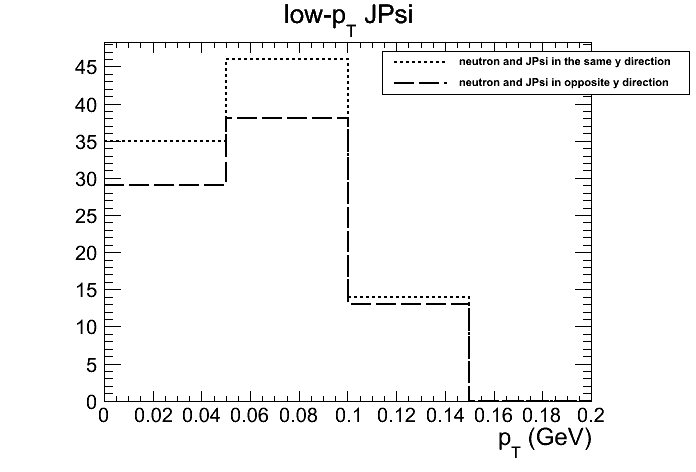
\includegraphics[angle=0,width=0.45\textwidth]{cohOppAndSameNeutronDir}
        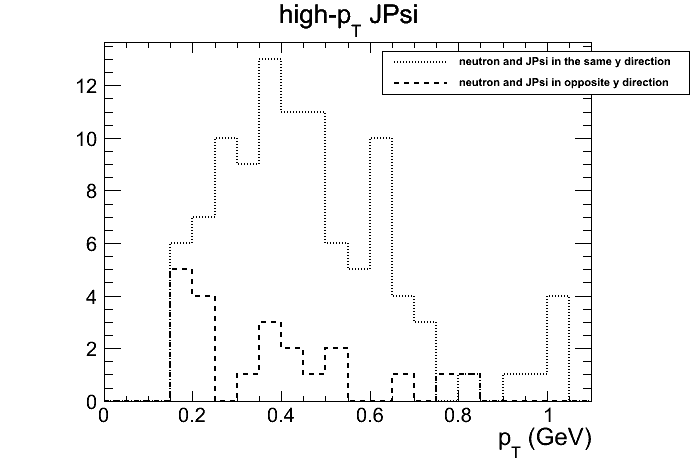
\includegraphics[angle=0,width=0.45\textwidth]{incohOppAndSameNeutronDir} \\
        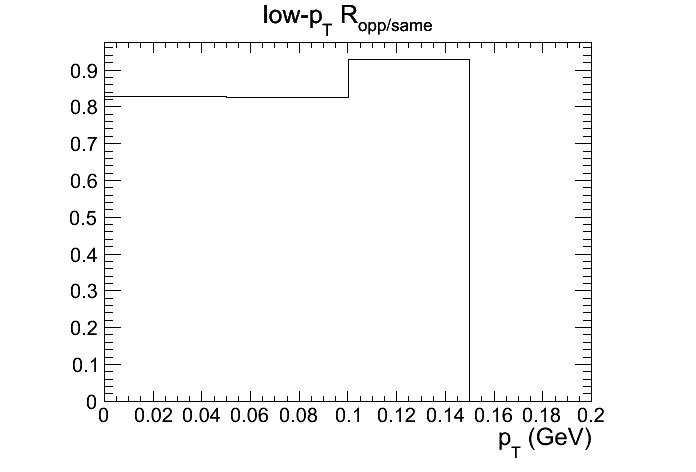
\includegraphics[angle=0,width=0.45\textwidth]{ratiocohOppAndSameNeutronDir}
        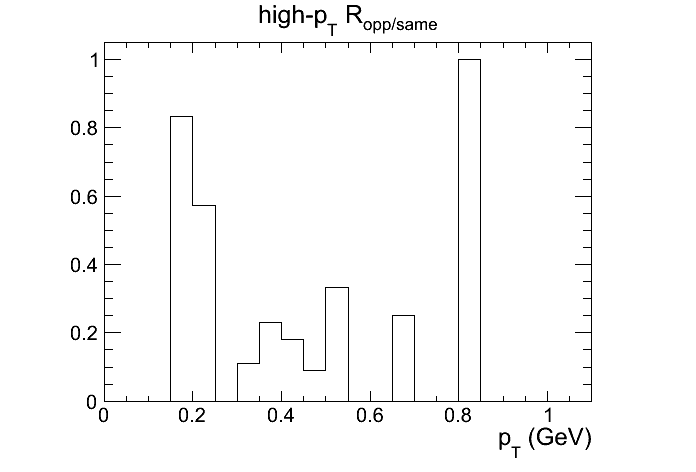
\includegraphics[angle=0,width=0.45\textwidth]{ratioincohOppAndSameNeutronDir}
      \caption{ \label{fig:PtcorrandRation}  
        Transverse momentum distribution of the $J/\psi$ when  $J/\psi$ and 
          neutron have the opposite rapidity direction and the transverse 
          momentum distribution of the $J/\psi$ when  $J/\psi$ and neutron
          have the same rapidity direction for low-\pt (top left) and 
          high-\pt (top right) \JPsi. Bottom: Ratios $R_{opp/same}$ for 
          low-\pt ( left) and high-\pt ( right) \JPsi.}
      \end{center}
    \end{figure*}
    
    Compiled for \pt$<$1.05~GeV $R_{opp/same}$ ratio between the \pt 
      distribution of the \JPsi having neutron emitted in the opposite 
      direction and  the \JPsi having the neutron emitted in the same
      direction is shown on Fig.~\ref{fig:r2}. 
    \begin{figure*}[!Hhtb]
      \begin{center}
        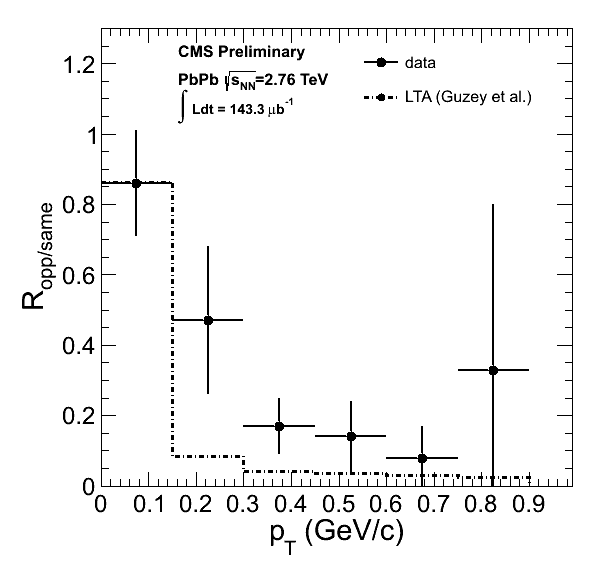
\includegraphics[angle=0,width=0.65\textwidth]{RoppsameVsTheory}
        \caption{ \label{fig:r2} Ratio between the transverse momentum 
          distribution of the $J/\psi$ when  $J/\psi$ and neutron have 
          the opposite direction and the transverse momentum distribution 
          of the $J/\psi$ when  $J/\psi$ and neutron have the same direction.}
      \end{center}
    \end{figure*}
    The same distributions as~\ref{fig:PtcorrandRation} but now as a function 
      of rapidity of the \JPsi are presented in the Fig~\ref{fig:r3} and 
      compiled in Fig.~\ref{fig:r4}. 
    
    \begin{figure*}[!Hhtb]
      \begin{center}
        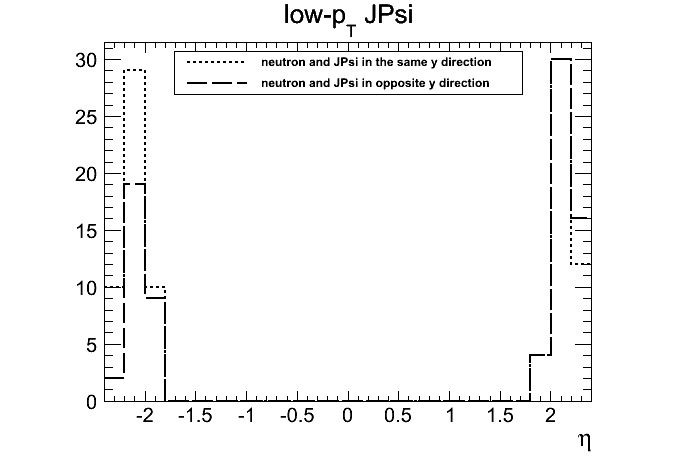
\includegraphics[angle=0,width=0.45\textwidth]{cohyOppAndSameNeutronDir}
        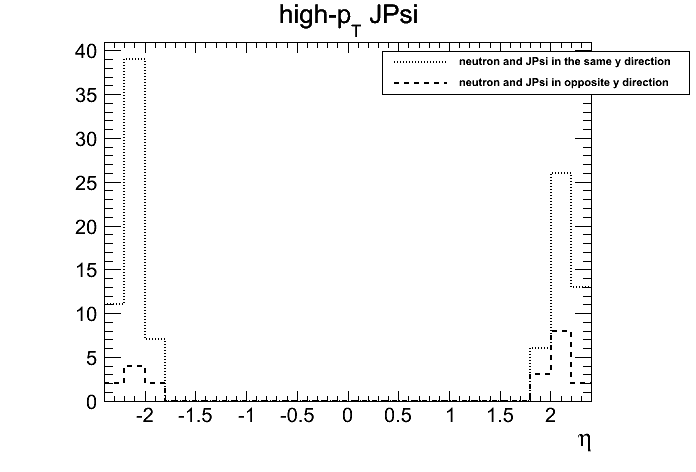
\includegraphics[angle=0,width=0.45\textwidth]{incohyOppAndSameNeutronDir}\\
        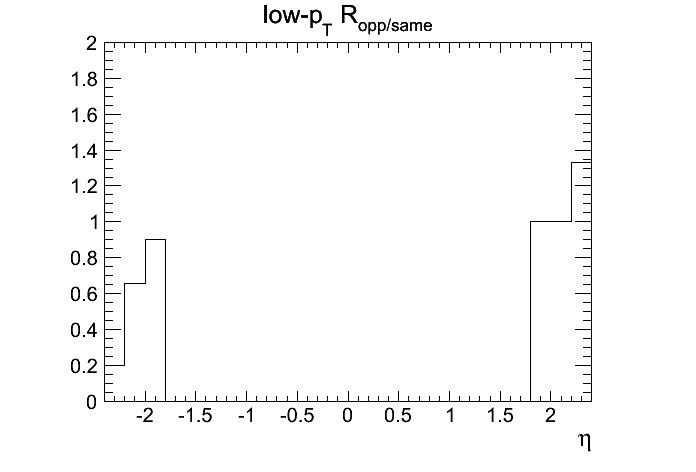
\includegraphics[angle=0,width=0.45\textwidth]{ratiocohyOppAndSameNeutronDir}
        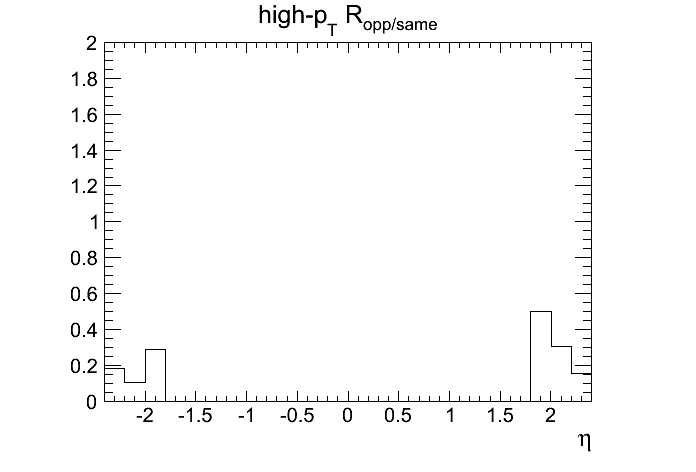
\includegraphics[angle=0,width=0.45\textwidth]{ratioincohyOppAndSameNeutronDir}
        \caption{ \label{fig:r3} Rapidity distribution of the $J/\psi$ when  
          $J/\psi$ and neutron have the opposite rapidity direction and the 
          rapidity distribution of the $J/\psi$ when  $J/\psi$ and neutron 
          have the same rapidity direction for low-\pt (top left) and high-\pt 
          (top right) \JPsi. Bottom: Ratios $R_{opp/same}$ for low-\pt ( left) 
          and high-\pt ( right) \JPsi.}
      \end{center}
    \end{figure*}
    
    \begin{figure*}[!Hhtb]
      \begin{center}
        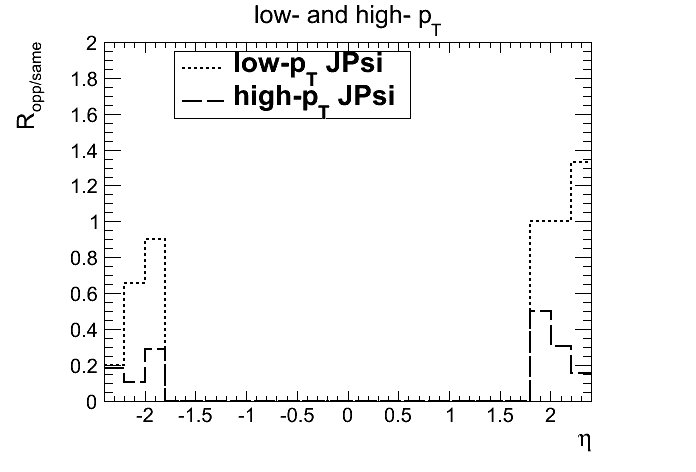
\includegraphics[angle=0,width=0.55\textwidth]{compiledratioincohandcohyOppAndSameNeutronDir}
        \caption{ \label{fig:r4} Rapidity ratios $R_{opp/same}$ for low-\pt 
          ( left) and high-\pt ( right) \JPsi.}
      \end{center}
    \end{figure*}
    
    Figure~\ref{fig:rNeutDimuCorr} shows the rapidity of the dimuon for the 
      events that are tagged by the ZDC$^{+}$ and  ZDC$^{-}$ means having 
      the neutron emitted in the $y>0$ and $y<0$. 
    
    \begin{figure*}[!Hhtb]
      \begin{center}
        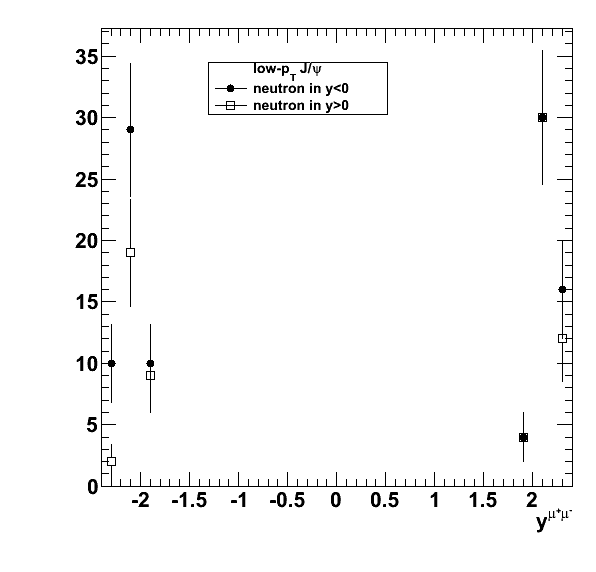
\includegraphics[angle=0,width=0.42\textwidth]{ZDCDimuCorrCoh}\\
        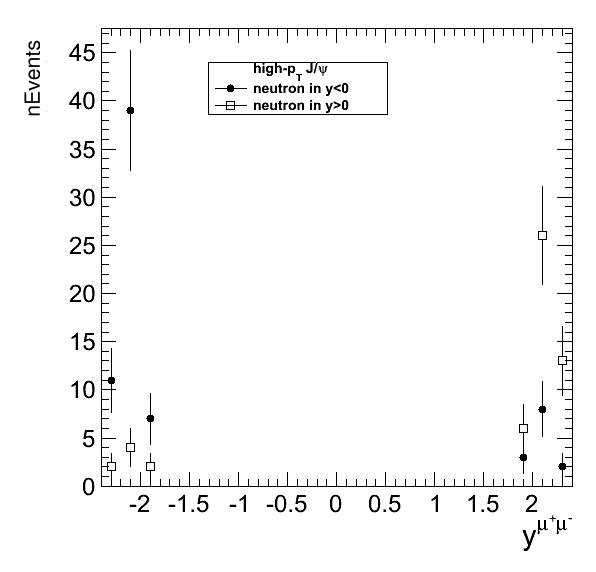
\includegraphics[angle=0,width=0.42\textwidth]{ZDCDimuCorrIncoh}\\
        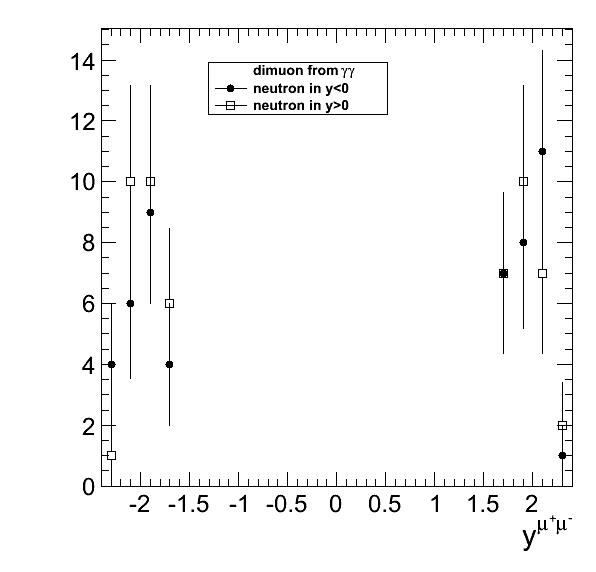
\includegraphics[angle=0,width=0.42\textwidth]{ZDCDimuCorrGammaGamma}
        \caption{ \label{fig:rNeutDimuCorr} Rapidity distribution of \JPsi in the
          case of the events having the neutron in negative and positive rapidity 
          for the low-\pt \JPsi (top), high-\pt \JPsi (middle) and dimuons from
          $\gamma \gamma$ sample (bottom). }
      \end{center}
    \end{figure*}
    
    Another, interesting correlation between the \JPsi rapidity direction and 
      the neutron rapidity can be also studied with quantities defined in 
      Eq.~\ref{eq:Ration} that are calculated in the 
      Table~\ref{tab:corrneutronjpsi}. 
    Table~\ref{tab:corrneutronjpsieffcorr} gives the same quantities as  
      Table.~\ref{tab:corrneutronjpsi} but here it is corrected for the 
      difference between the efficiency of the ZDC$^{+}$ and  ZDC$^{-}$. 
    
    \begin{equation}
      \label{eq:Ration}
      R_{(\mu\mu)^{-}}^{n^{-}/n^{+}} =  \frac{y^{-}_{\mu\mu} \wedge 
        y_{n}^{-}}{y^{-}_{\mu\mu} \wedge y_{n}^{+} }~~~~~~~~\mbox{and}~~~~~
        R_{(\mu\mu)^{+}}^{n^{-}/n^{+}} =  \frac{y^{+}_{\mu\mu} \wedge 
        y_{n}^{-}}{y^{+}_{\mu\mu} \wedge y_{n}^{+} }
    \end{equation}
    
    \begin{table}[h]
      \begin{center}
        \begin{tabular}{|c|c|c|c|c|c|c|}
          \hline
          & $y^{-}_{\mu\mu} \wedge y_{n}^{-}$ & $y^{-}_{\mu\mu} \wedge y_{n}^{+}$ 
          & $y^{+}_{\mu\mu} \wedge y_{n}^{+}$ & $y^{+}_{\mu\mu} \wedge y_{n}^{-}$ 
          & $R_{(\mu\mu)^{-}}^{n^{-}/n^{+}}$ 
          & $R_{(\mu\mu)^{+}}^{n^{-}/n^{+}} $  \\ \hline
          low-\pt \JPsi & \textcolor{blue}{78 $\pm$ 8.8} 
          & \textcolor{blue}{47 $\pm$  6.8}  & \textcolor{blue}{81 $\pm$  9}  
          & \textcolor{blue}{74 $\pm$  8.6} & \textcolor{blue}{ 1.66$\pm$0.31  } 
          & \textcolor{blue}{ 0.91$\pm$0.15  } \\ \hline
          high-\pt \JPsi & \textcolor{blue}{132 $\pm$  11.5}  
          & \textcolor{blue}{17 $\pm$  4.1}  & \textcolor{blue}{117 $\pm$  10.8}  
          & \textcolor{blue}{29 $\pm$  5.4} & \textcolor{blue}{7.76$\pm$2.0} 
          & \textcolor{blue}{0.25$\pm$0.05 } \\ \hline
          $\mu^{+}\mu^{-}$ from $\gamma \gamma$ & \textcolor{blue}{80 $\pm$8.9} 
          & \textcolor{blue}{81 $\pm$9} & \textcolor{blue}{75 $\pm$8.7} 
          & \textcolor{blue}{83 $\pm$9.1} & \textcolor{blue}{0.99$\pm$0.16 } 
          & \textcolor{blue}{1.11$\pm$0.18} \\ \hline
        \end{tabular}
        \caption{\label{tab:corrneutronjpsi} Number of dimuon pairs for 
          different directions of the neutron rapidity direction together with 
          $R_{(\mu\mu)^{-}}^{n^{-}/n^{+}}$ and 
          $R_{(\mu\mu)^{+}}^{n^{-}/n^{+}}$.}
      \end{center}
    \end{table}
    
    \begin{table}[h]
      \begin{center}
        \begin{tabular}{|c|c|c|}
          \hline
          & $R_{(\mu\mu)^{-}}^{\varepsilon_{ZDC}(n^{-}/n^{+})}$ 
          & $R_{(\mu\mu)^{+}}^{\varepsilon_{ZDC}(n^{-}/n^{+})} $  \\ \hline
          low-\pt \JPsi &  \textcolor{blue}{1.59 $\pm$ 0.29} 
          & \textcolor{blue}{0.88 $\pm$ 0.14} \\ \hline
          high-\pt \JPsi  & \textcolor{blue}{7.45 $\pm$ 1.87}  
          &  \textcolor{blue}{0.24 $\pm$ 0.05 } \\ \hline
          $\mu^{+}\mu^{-}$ from $\gamma \gamma$ 
          & \textcolor{blue}{0.95 $\pm$ 0.15} 
          & \textcolor{blue}{ 1.06 $\pm$ 0.17 } \\ \hline
        \end{tabular}
        \caption{\label{tab:corrneutronjpsieffcorr} Ratios 
          $R_{(\mu\mu)^{-}}^{\varepsilon_{ZDC}(n^{-}/n^{+})}$ and 
          $R_{(\mu\mu)^{+}}^{\varepsilon_{ZDC}(n^{-}/n^{+})} $ 
          i.e. $R_{(\mu\mu)^{-}}^{n^{-}/n^{+}}$ and 
          $R_{(\mu\mu)^{+}}^{n^{-}/n^{+}} $ corrected by the ZDC$^{+}$ and
          ZDC$^{-}$ efficiencies.}
      \end{center}
    \end{table}
    
    Integrated over rapidity, separately for $y<0$ and $y>0$ ratios from 
      Table~\ref{tab:corrneutronjpsieffcorr} are shown in the 
      Figure~\ref{fig:integRatios}.
    
    \begin{figure*}[!Hhtb]
      \begin{center}
        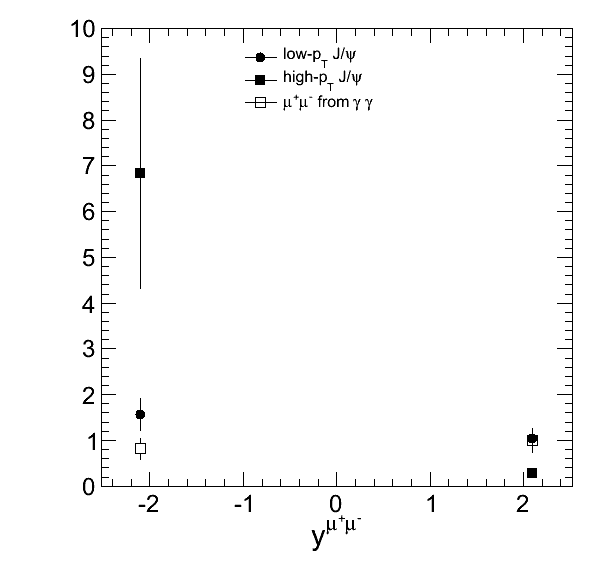
\includegraphics[angle=0,width=0.52\textwidth]{RCompiledYCorr}
        \caption{ \label{fig:integRatios} 
          $R_{(\mu\mu)^{-}}^{\varepsilon_{ZDC}(n^{-}/n^{+})}$ and 
          $R_{(\mu\mu)^{+}}^{\varepsilon_{ZDC}(n^{-}/n^{+})}$ integrated over 
          one side in rapidity for low- and high-\pt \JPsi and also for dimuons
          from $\gamma \gamma$ sample. }
      \end{center}
    \end{figure*}
    
    From the Tab~\ref{tab:corrneutronjpsi} and the Fig.~\ref{fig:rNeutDimuCorr} 
      it is seen as expected that there is no correlation between the \JPsi 
      rapidity and neutron rapidity in the case of the low-\pt \JPsi and 
      dimuons coming from $\gamma \gamma$ sample. 
    In the case of the high-\pt \JPsi the correlation is clearly visible.  
